% =========================================================
% CONFIGURACION DEL DOCUMENTO
% =========================================================
\providecommand{\main}{../..}
\documentclass[\main/main.tex]{subfiles}

% =========================================================
% CONTENIDO
% =========================================================
\begin{document}
\section{Diseño de Control Estabilizador}\label{Diseo de Control Estabilizador}
\subsection{Sistema lineal}

El objetivo principal de este trabajo es la estabilización en vuelo
hovering del vehículo. Para ésto, se tienen en consideración los angulos
roll, pitch y yaw $(\phi,\ \theta,\ \psi)$ únicamente, puesto que
si bien es de interés para la prueba en vuelo controlar la altura,
en primera instancia se desea controlar las orientaciones en estos
tres ángulos sobre un soporte con los tres grados de libertad correspondientes.
Sin embargo, para la simulación del sistema también se controla la
altura del vehículo, por lo cual se incluirán las consideraciones
necesarias para realizarlo.

En primer lugar se dejan expresadas los momentos y la fuerza de empuje
descritas en el capítulo de modelado en función de las velocidades
angulares de los cuatro rotores:

\begin{equation}
u=K_{T}\cdot(\omega_{1}^{2}+\omega_{2}^{2}+\omega_{3}^{2}+\omega_{4}^{2})
\end{equation}

\begin{equation}
u_{1}=\tau_{\phi}=\ell\cdot(f_{2}-f_{4})=K_{T}\cdot(\omega_{2}^{2}-\omega_{4}^{2})\cdot\ell
\end{equation}

\begin{equation}
u_{2}=\tau_{\theta}=\ell\cdot(f_{3}-f_{1})=K_{T}\cdot(\omega_{3}^{2}-\omega_{1}^{2})\cdot\ell
\end{equation}

\begin{equation}
u_{3}=\tau_{\psi}=\sum_{i=1}^{4}\tau_{M_{i}}=K_{M}\cdot(\omega_{1}^{2}-\omega_{2}^{2}+\omega_{3}^{2}-\omega_{4}^{2})
\end{equation}

Donde $\ u_{1},\ u_{2},\ u_{3}$ son las entradas para el control
estabilizador. 

Dado el vector de entradas $\vec{u}=[u\ u_{1}\ u_{2}\ u_{3}]$, se
linealiza el sistema descrito por la ecuación  (\ref{eq:141}) en torno a un punto
de operación $\vec{x}=[\eta,\ W_{\eta}\dot{\eta}]=[\vec{0},\ \vec{0}]$
para pequeñas oscilaciones, es decir se aproxima la función seno del
ángulo al argumento y coseno del ángulo a la unidad. Esta aproximación
es válida para valores pequeños del argumento, lo que concuerda con
el propósito de estabilización en hovering.

De la ecuación (\ref{eq:138}) se tiene:

\[
\begin{bmatrix}\dot{\phi}\\
\dot{\theta}\\
\dot{\psi}
\end{bmatrix}=\begin{bmatrix}p+r\cdot cos\phi tan\theta+q\cdot sen\phi tan\theta\\
q\cdot cos\phi-r\cdot sen\phi\\
r\cdot\frac{cos\phi}{cos\theta}+q\cdot\frac{sen\phi}{cos\theta}
\end{bmatrix}
\]


Al simplificar las expresiones por la aproximación a pequeña oscilación
se tiene:

\[
\begin{bmatrix}\dot{\phi}\\
\dot{\theta}\\
\dot{\psi}
\end{bmatrix}=\begin{bmatrix}p+r\theta+q\phi\theta\\
q-r\phi\\
r+q\phi
\end{bmatrix}
\]


Por lo tanto el modelo no lineal es:

\[
\begin{bmatrix}\dot{\phi}\\
\dot{\theta}\\
\dot{\psi}\\
\dot{p}\\
\dot{q}\\
\dot{r}
\end{bmatrix}=\begin{bmatrix}p+r\theta+q\phi\theta\\
q-r\phi\\
r+q\phi\\
(I_{y}-I_{z})qr/I_{x}+\tau_{\phi}/I_{x}\\
(I_{z}-I_{x})pr/I_{y}+\tau_{\theta}/I_{y}\\
(I_{x}-I_{y})pq/I_{z}+\tau_{\psi}/I_{z}
\end{bmatrix}=f(\vec{x},\vec{u})
\]

Linealizando el modelo a pequeña oscilación en torno al punto de operación
$\vec{x}=[\eta,\ W_{\eta}\dot{\eta}]=[\vec{0},\ \vec{0}]\in\mathbb{R}^{6}$
y a la entrada constante en el punto de equilibrio $\vec{u}=[u,\,0,\,0,\,0]\in\mathbb{R}^{4}$,
se obtiene el siguiente modelo:

\[
\dot{\triangle x}=A\cdot\triangle x+B\cdot\triangle u
\]
\[
A=\frac{\partial f(\vec{x},\vec{u})}{\partial\vec{x}}\bigg|_{\vec{x}=\vec{0},\,\vec{u}=\vec{0}}=\begin{bmatrix}0 & 0 & 0 & 1 & 0 & 0\\
0 & 0 & 0 & 0 & 1 & 0\\
0 & 0 & 0 & 0 & 0 & 1\\
0 & 0 & 0 & 0 & 0 & 0\\
0 & 0 & 0 & 0 & 0 & 0\\
0 & 0 & 0 & 0 & 0 & 0
\end{bmatrix}
\]


\[
B=\frac{\partial f(\vec{x},\vec{u})}{\partial\vec{u}}\bigg|_{\vec{x}=\vec{0},\,\vec{u}=\vec{0}}=\begin{bmatrix}0 & 0 & 0 & 0 & 0 & 0\\
0 & 0 & 0 & 0 & 0 & 0\\
0 & 0 & 0 & 0 & 0 & 0\\
0 & 0 & 0 & 1/I_{x} & 0 & 0\\
0 & 0 & 0 & 0 & 1/I_{y} & 0\\
0 & 0 & 0 & 0 & 0 & 1/I_{z}
\end{bmatrix}
\]


\[
\begin{bmatrix}\dot{\triangle\phi}\\
\dot{\triangle\theta}\\
\dot{\triangle\psi}\\
\dot{\triangle p}\\
\dot{\triangle q}\\
\dot{\triangle r}
\end{bmatrix}=\begin{bmatrix}\triangle p\\
\triangle q\\
\triangle r\\
\triangle\tau_{\phi}/I_{x}\\
\triangle\tau_{\theta}/I_{y}\\
\triangle\tau_{\psi}/I_{z}
\end{bmatrix}
\]

Es claro que el sistema simplificado es lineal y desacoplado, por
lo tanto se pueden utilizar técnicas de control lineal para propósitos
de estabilización de los ángulos. 

En primer lugar se calculan las funciones de transferencia de cada
uno de los ángulos de inclinación del vehículo.

\[
H_{\phi}(s)=\frac{1}{I_{xx}}\cdot\frac{1}{s^{2}}\qquad H_{\theta}(s)=\frac{1}{I_{yy}}\cdot\frac{1}{s^{2}}\qquad H_{\psi}(s)=\frac{1}{I_{zz}}\cdot\frac{1}{s^{2}}
\]

Por lo tanto cada una de las funciones de transferencia son de segundo
orden e inestables, ya que poseen dos polos en el origen del plano
complejo. El diagrama para cada función de transferencia y el lugar
geométrico de raíces para cada una, se muestran a continuación.

\begin{figure}[H]
\noindent \begin{centering}
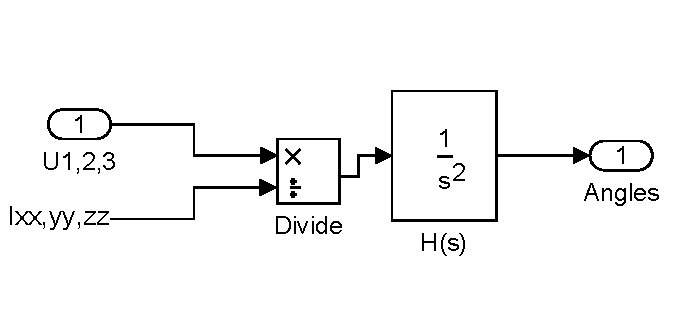
\includegraphics[scale=0.6]{Transferencias}
\par\end{centering}
\caption{Diagrama de transferencias de lazo abierto.}
\end{figure}

\begin{figure}[H]
\noindent \begin{centering}
\includegraphics[scale=0.75]{\string"sisotool tranferencias\string".pdf}
\par\end{centering}
\caption{Lugar Geométrico de Raíces en Lazo Abierto de $H_{\phi,\theta,\psi}(s)$.}
\end{figure}

\subsection{Diseño de Controlador}

\subsubsection{Control Estabilizador}

Para el diseño de la ley de control se deben considerar en primera
instancia las especificaciones de desempeño. Por lo general las especificaciones
de desempeño no deben ser más rigurosas de lo necesario para cumplir
con el objetivo definido, puesto que al incrementar las exigencias,
incrementan los conflictos o compromisos entre los parámetros a sintonizar,
o bien, conducen a un desarrollo muy costoso. Por lo tanto las especificaciones
principales del diseño son estabilizar el sistema, además de realizar
seguimiento de referencias constantes para altura y ángulos pitch,
roll y yaw, y por último, generar una respuesta transitoria lo más
rápida posible. 

El lazo de control a implementar en la simulación es el siguiente:

\begin{figure}[H]
\noindent \begin{centering}
\includegraphics[scale=0.5]{\string"arquitectura de contro\string".jpg}
\par\end{centering}
\caption{\label{fig:Esquema-de-Com}Esquema de Control Seleccionado.}
\end{figure}

Para el diseño de la ley de control se utiliza un controlador de la
familia de controladores PID. Las principales ventajas de los controladores
PID son su estructura simple y facilidad para la implementación. 

En primer lugar se describe el funcionamiento básico de esta familia
de controladores. Se considera el lazo de una entrada y una salida
(SISO) como el de la figura \ref{fig:Esquema-de-Com}, analizando una función
de transferencia generalizada para los ángulos, dado que son prácticamente
iguales salvo por la constante que aporta la matriz de inercia. 

Los controladores de la familia PID incluyen tres acciones: Proporcional,
Integrativa y Derivativa. 

\begin{itemize}
\item $P:\ acci\acute{o}n\ proporcional:$ entrega una salida de control
proporcional al error entre la referencia y la variable a controlar,
es decir $u(t)=K_{p}e(t)$. Por lo tanto su transferencia es simplemente
una ganancia 
\[
C_{p}(s)=K_{p}=\frac{U(s)}{E(s)}
\]
\end{itemize}

\begin{itemize}
\item $I:\ acci\acute{o}n\ integral:$ entrega una salida de control que
es proporcional a la integral del error acumulado. Por el teorema
del valor final, agregar integración a controladores, implica obtener
un error estacionario cero en referencias constantes, siempre y cuando el lazo sea estable en lazo cerrado.

\[
u(t)=\frac{1}{K_{i}}\intop_{0}^{t}e(\tau)d\tau\hfill C_{i}=\frac{1}{K_{i}s}=\frac{U(s)}{E(s)}
\]

\item $PI:\ acci\acute{o}n\ proporcional\ integrativa:$ es la combinación
de las acciones descritas anteriormente. Con la acción proporcional
si el error es cero en cierto instante, también lo es su acción. Mientras
que con la acción integral, si existe error por pequeño que sea, siempre
se tendrá actuación creciente o decreciente dependiendo del signo
de dicho error. Sus expresiones en el tiempo y como función de transferencia
son:
\[
u(t)=K_{p}e(t)+\frac{1}{K_{i}}\intop_{0}^{t}e(\tau)d\tau\hfill C_{PI}=K_{p}+\frac{1}{K_{i}s}=\frac{U(s)}{E(s)}
\]
\end{itemize}

 
\begin{itemize}
\item $PD:\ acci\acute{o}n\ proporcional\ derivativa:$ Se define como 
\[
u(t)=K_{p}e(t)+K_{d}\frac{de(t)}{dt}\hfill C_{PD}(s)=K_{p}+K_{d}s=\frac{U(s)}{E(s)}
\]
\end{itemize}

Esta acción agrega rapidez a la respuesta del lazo cerrado, puesto
que sensibiliza al lazo respecto de las variaciones en el error, aplicando
correcciones oportunas antes que la magnitud del mismo crezca de forma
vigorosa. Sin embargo también cuenta con algunas desventajas, suele
amplificar la acción de control o actuación hasta el punto de saturación
en algunos casos, además de amplificar el ruido. La acción derivativa
rara vez se utiliza por si sóla, dado que es de utilidad sólo por
cortos periodos de tiempo. 
\begin{itemize}
\item $PID:\ acci\acute{o}n\ proporcional-integrativa-derivativa:$ Esta
acción combina las ventajas de cada una de las acciones de control
descritas con anterioridad y sus expresiones son las siguientes:
\[
u(t)=K_{p}e(t)+\frac{1}{K_{i}}\intop_{0}^{t}e(\tau)d\tau+K_{d}\frac{de(t)}{dt}
\]
\end{itemize}
\[
C_{PID}(s)=K_{p}+\frac{1}{K_{i}s}+K_{d}s=\frac{U(s)}{E(s)}
\]

Una vez descritas las principales acciones de control, se debe seleccionar
un controlador de la gama PID. Para esto se calculan las diferentes
funciones de sensibilidad de lazo cerrado para cada controlador, ignorando
los bloques de prealimentación de la referencia y filtrado del ruido
de medición.
\begin{itemize}
\item $P:\ acci\acute{o}n\ proporcional:$ Se calcula la función de sensibilidad
que relaciona la referencia con la salida del lazo cerrado
\[
T_{o}(s)=\frac{G_{o}(s)C(s)}{1+G_{o}(s)C(s)}=\frac{K_{p}/I_{eje}}{s^{2}+\frac{1}{I_{eje}}}
\]
\end{itemize}

Es claro que una acción proporcional no es suficiente, dado que los
polos de la función de sensibilidad están ubicados en el eje imaginario
$s=\pm\frac{j}{I_{eje}}$, por lo tanto el lazo cerrado es inestable.

\begin{itemize}
\item $PI:\ acci\acute{o}n\ proporcional\ integrativa:$ La función de sensibilidad
$T_{o}$ es:
\[
T_{o}(s)=\frac{G_{o}(s)C(s)}{1+G_{o}(s)C(s)}=\frac{K_{P}s+K_{i}}{I_{eje}s^{3}+K_{p}s+K_{i}}
\]
\end{itemize}

Analizando la estabilidad de la función de sensibilidad $T_{o}(s)$,
se buscan los polos con $K_{p}=0.$ Se utiliza el comando $root$
de $MATLAB$, definiendo como variables simbólicas a la constante
de inercia $I_{eje}$ y la acción integral $K_{i}$. Los polos de
la función de sensibilidad son:

\[
s_{1}=-\sqrt[3]{\frac{K_{i}}{I_{eje}}}\qquad s_{2}=\sqrt[3]{\frac{K_{i}}{I_{eje}}}\cdot(\frac{1}{2}-\frac{\sqrt{3}}{2}j)\qquad s_{3}=\sqrt[3]{\frac{K_{i}}{I_{eje}}}\cdot(\frac{1}{2}+\frac{\sqrt{3}}{2}j)
\]

Por lo tanto si $K_{i}>0$ se tiene dos polos complejos conjugados
en el semiplano derecho y si $K_{i}<0$ existe un polo real en el
semiplano derecho. Por lo tanto la función de sensibilidad es inestable
para $K_{p}=0$. 

Luego se analiza el comportamiento en lazo cerrado para $K_{p}\neq0$
utilizando el toolbox $sisotool$, el cual permite visualizar el lugar
geométrico de raices en función de los parámetros del controlador,
de forma más eficiente que un análisis de las expresiones que son
solución del $Acl=0$ correspondiente al denominador de la función
de sensibilidad. Para el análisis se utiliza un valor para la componente
de la matriz de inercia $I_{eje}=0.0048$, calculado en el capítulo
de simulación, correspondiente a la inercia del vehículo sobre el
eje $y$, por lo tanto la transferencia corresponde al giro en el
ángulo $\theta$ pitch. Se analiza sólo un caso dada la similitud
entre las transferencias.

\begin{figure}[H]
\noindent \begin{centering}
\subfloat[LGR Lazo Cerrado, Control PI, Parámetros 1.\label{fig:LGR-Lazo-Cerrado PI1}]{\noindent \begin{centering}
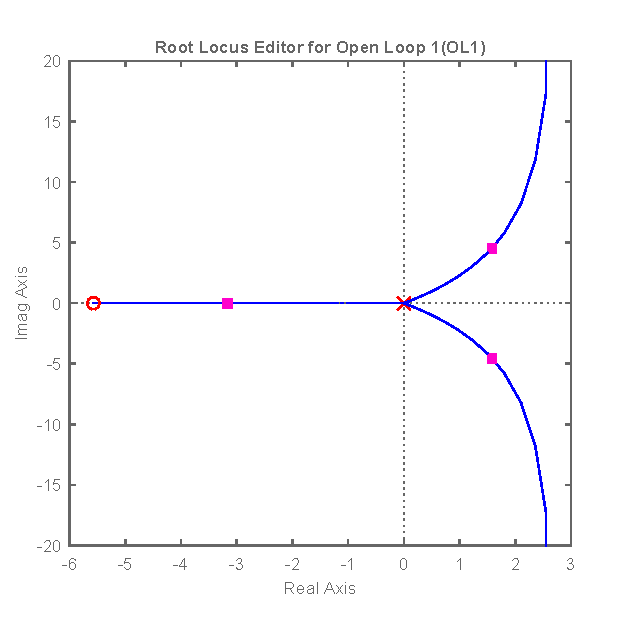
\includegraphics[scale=0.6]{Ti_PI_Control1}
\par\end{centering}
}\subfloat[LGR Lazo Cerrado, Control PI, Parámetros 2.\label{fig:LGR-Lazo-Cerrado PI2}]{\noindent \begin{centering}
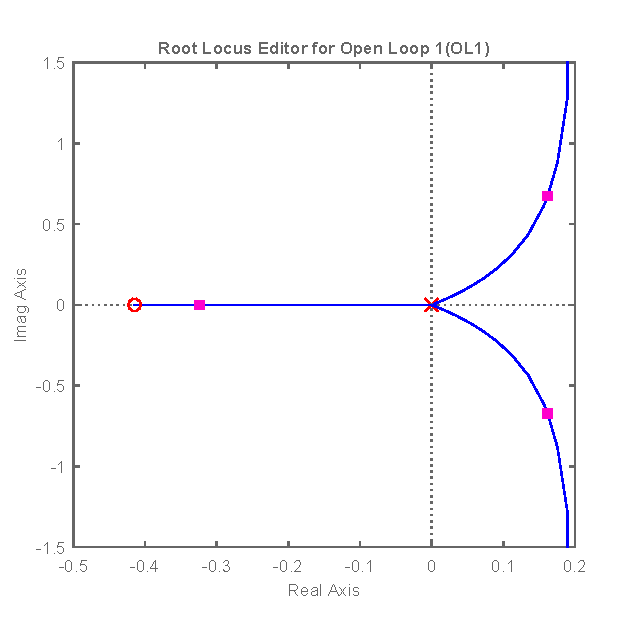
\includegraphics[scale=0.6]{To_PI_Control2}
\par\end{centering}}
\par\end{centering}
\caption{LGR en Lazo Cerrado de Planta Lineal con Control PI para diferentes
parámetros.}
\end{figure}

Para el gráfico de la figura \ref{fig:LGR-Lazo-Cerrado PI1} los parámetros
son $K_{p}=0.1119$ y $K_{i}=0.6216$, mientras que para la figura
\ref{fig:LGR-Lazo-Cerrado PI2} son $K_{p}=0.0031$ y $K_{i}=0.0013$.
De ambas figuras se puede concluir que para diferentes valores de
los parámetros, el cero real se acerca o se aleja del origen atrayendo
a un polo hacia él, pero los polos complejos conjugados siempre se
encuentran en el semiplano derecho, por lo tanto el sistema es inestable
para este tipo de controlador.
\begin{itemize}
\item $PD:\ acci\acute{o}n\ proporcional\ derivativa:$ La función de sensibilidad
$T_{o}$ es:
\end{itemize}
\[
T_{o}(s)=\frac{G_{o}(s)C(s)}{1+G_{o}(s)C(s)}=\frac{K_{p}+K_{d}s}{I_{eje}s^{2}+K_{d}s+K_{p}}
\]

Analizando la función de sensibilidad $T_{o}(s)$ es claro que se
puede estabilizar el sistema escogiendo los parámetros $K_{d}$ y
$K_{p}$ ambos mayores que cero, sin embargo, es conveniente de todas
formas analizar el Lugar Geométrico de Raíces para buscar los parámetros
que den mayor rapidez al lazo. 

El Lugar Geométrico de Raíces de la planta con controlador PD para
un cero real en el semi plano izquierdo, es el siguiente:

\begin{figure}[H]
\noindent \begin{centering}
\includegraphics[scale=0.8]{\string"LGR PD\string".pdf}
\par\end{centering}
\caption{LGR Control PD sin filtro de primer orden. $C(s)=3\cdot(1+s)$.}
\end{figure}

Como el controlador previamente diseñado posee grado relativo menor
que uno, en teoría no es posible su implementación. Debido a esto,
también se estudia un controlador PD con filtro derivativo de primer
orden. 

\[
T_{o}(s)=\frac{G_{o}(s)C(s)}{1+G_{o}(s)C(s)}=\frac{K_{p}+K_{d}s}{I_{eje}s^{3}+\alpha I_{eje}s^{2}+K_{d}s+K_{p}}
\]

El Lugar Geométrico de Raices de este controlador depende de la posición
relativa del cero real y el polo real en el semiplano izquierdo. En
primer lugar se ubica el cero real a la izquierda del polo real, por
lo cual el sistema es inestable, dado que los polos inestables de
la planta siempre quedan en el semiplano derecho del plano complejo. 

\begin{figure}[H]
\noindent \begin{centering}
\includegraphics[scale=0.8]{\string"LGR PD filtro derivativo\string".pdf}
\par\end{centering}
\caption{LGR Control PD con filtro derivativo de primer orden, sistema inestable.}
\end{figure}

Luego se diseña el controlador ubicando el polo real a la derecha
del cero real, aumentando la ganancia para que los polos inestables
de la planta se alejen del eje imaginario. Con esta configuración
el lazo es estable y robusto a pequeñas perturbaciones. 

\begin{figure}[H]
\noindent \begin{centering}
\includegraphics[scale=0.8]{\string"LGR PD filtro derivativo estable\string".pdf}
\par\end{centering}
\caption{LGR con filtro derivativo de primer orden, sistema estable. $C(s)=\frac{(42.87+8.574s)}{(100+s)}$ }
\end{figure}

\begin{itemize}
\item $PID:\ acci\acute{o}n\ proporcional,\ Integral\ y\ derivativa:$ La
función de sensibilidad $T_{o}$ es:
\end{itemize}
\[
T_{o}(s)=\frac{G_{o}(s)C(s)}{1+G_{o}(s)C(s)}=\frac{K_{d}K_{i}s^{2}+K_{p}K_{i}s+1}{(I_{eje}K_{i}+K_{d}K_{i})s^{2}+K_{p}K_{i}s+1}
\]


Analizando la función de sensibilidad $T_{o}(s)$ se puede observar
que si los parámetros del controlador se escojen todos mayores que
cero, el lazo de control es estable. 

\begin{figure}[H]
\noindent \begin{centering}
\includegraphics[scale=0.8]{\string"LGR PID estable\string".pdf}
\par\end{centering}
\caption{LGR Control PID, sistema estable.}
\end{figure}

La principal desventaja de implementar el control PID, es la acción integral del controlador y su efecto en la actuación del sistema, mejor conocido como wind-up. 
En algunos casos el wind-up produce oscilaciones sostenidas en vez de estabilización, junto con un mayor tiempo en alcanzar la estabilidad. En otros casos produce inestabilidad. 
Después de analizar cada controlador por seaparado, se decide implementar
un controlador PD para la simulación, dado que estabiliza el sistema
en vuelo hovering de mejor manera. 

\subsubsection{Control de Altura}

Para controlar la altura del vehículo se toma en cuenta la ecuación
que describe la aceleración en el eje Z descrita anteriormente en
el capítulo de modelado:

\[
\ddot{z}=-g+\frac{u}{m}Cos(\theta)Cos(\phi)
\]

Dicha dinámica es no lineal y multivariable, pues depende de las mediciones
de los ángulos para proyectar el empuje total sobre el eje Z. Por
eso se aborda el problema de control con una estrategia diferente,
diseñando una entrada de empuje ad-hoc para mantener el vehículo con
una altura constante.

Si el requerimiento es que el quadcopter se mantenga en vuelo hovering
en pequeñas perturbaciones, basta con hacer el empuje total igual
al peso del vehículo y distribuir dicho empuje entre los cuatro motores.
Sin embargo, dado que en la simulación y en la realidad el vehículo
puede ser sometido a perturbaciones mayores, se debe igualar la proyección
del empuje sobre el eje Z, a partir de la medición de los ángulos.
Por lo tanto, el empuje deseado es:

\[
u=\frac{mg}{Cos(\theta)Cos(\phi)}
\]

Dado que el empuje total es la suma del empuje realizado por cada
motor, se tiene:

\[
\sum_{i=1}^{4}u_{i}=\frac{mg}{Cos(\theta)Cos(\phi)}
\]

Y como el empuje es directamente proporcional a la velocidad angular
al cuadrado de cada motor:

\[
\sum_{i=1}^{4}\omega_{i}^{2}=\frac{mg}{K_{M}Cos(\theta)Cos(\phi)}
\]

Por lo tanto, si para cada motor se mantiene una velocidad igual a
la cuarta parte de la ecuación anterior, la altura del vehículo se
mantendrá constante. 

Luego si se quiere variar el setpoint de altura, en [13] se plantea
el siguiente esquema de control:

\[
u=(g+K_{z,\ D}(\dot{z}_{d\ ref}-\dot{z})+K_{z,\ P}(z_{ref}-z))\cdot\frac{m}{Cos(\theta)Cos(\phi)}
\]

El cual corresponde a un control PD al igual que en los casos anteriores,
pero genera un empuje de referencia a partir de la medición de dos
ángulos.

\end{document}